\section{Introduction}
Data are susceptible to various forms of corruption such as missing, incorrect, or inconsistent values.
Predictive modeling, such as regression and classification, are increasingly popular in data analytics \cite{bdas, alexandrov2014stratosphere, crotty2014tupleware, hellerstein2012madlib}.
These models can be highly sensitive to dirty data.
Predictive models rely on learning relationships between features and labels, and systematic corruption \cite{taylor1982introduction} (i.e., corruption that disproportionately affects certain data) can mask or even introduce spurious new relationships.
Furthermore, the high dimensionality of these models can amplify small problems resulting in error-prone predictions even when trained on mostly clean data \cite{xiaofeature}.

The challenge is that cleaning dirty data can be expensive, and analysts report that it is one of the most time consuming steps in the analysis process \cite{nytimes}.
Cleaning can require a significant amount of developer effort in writing software or rules to fix the corruption.
Furthermore, for data cleaning techniques that employ human validation or crowdsourcing, the actual cleaning operations can be costly for large datasets.
Analysts who want to train models on dirty data face a difficult choice between discarding the dirty data and inducing an unknown bias, or paying the price of data cleaning.

This paper explores techniques to train accurate models without having to clean the entire dataset.
In particular, we explore the problem of progressive data cleaning~\cite{altowim2014progressive, whang2014incremental, papenbrock2015progressive, gruenheid2014incremental, mayfield2010eracer, DBLP:journals/pvldb/YakoutENOI11, yakout2013don}, and formulate algorithms to incrementally update models given newly cleaned data.
There are a number of applications for such a framework including: early stopping when the model accuracy no longer improves, evaluating costly data cleaning without cleaning the entire dataset, and allowing for interactive data cleaning procedures.
These applications are only possible if the intermediate state of the model (based on $k \ll N$ clean records) is an accurate estimate of the true model.

Unfortunately, straight-forward implementations of progressive data cleaning can result in highly inaccurate models.
Training a model on a mixture of dirty and clean data can lead to misleading relationships in even simple scenarios (Figure \ref{update-arch1}).
An alternative is to restrict training to the $k$ records and to disregard all of the remaining dirty records (e.g., sampling \cite{wang1999sample}).
While this avoids the mixing problem, accurate model training may require a large amount of training data and $k$ examples may not be enough for a viable model.
Furthermore, if the $k$ records are not selected uniformly at random, the trained model might be highly biased.
The errors and inefficiencies introduced by these three problems may dominate any gains from data cleaning, leading to unreliable or misleading conclusions about data or model quality.

\begin{figure}[t]
\centering
 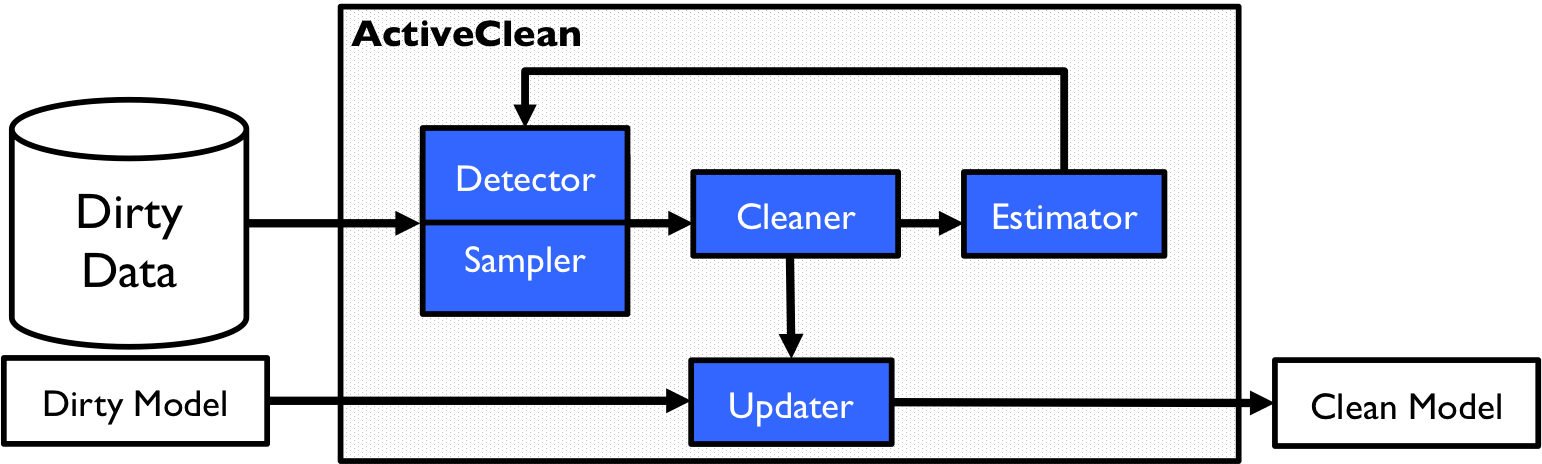
\includegraphics[width=\columnwidth]{figs/arch.png}
 \caption{\sysfull allows users to train predictive models while progressively cleaning data. The framework adaptively selects the best data to clean and can optionally (denoted with dotted lines) integrate with pre-defined detection rules and estimation algorithms for improved conference. \label{sys-arch}}\vspace{-2em}
\end{figure}

We present a system called \sys which applies progressive data cleaning with accuracy guarantees on predictive models trained after data cleaning.
We focus on two subproblems for a popular class of models called convex loss models (e.g., includes linear regression and SVMs): (1) the correctness problem of estimating and bounding the error in a model trained from dirty and clean data, and (2) the efficiency problem of actively selecting data to clean while preserving correctness.
We show that instead of re-training the model, the model should be incrementally maintained with gradient descent given newly cleaned data, an technique that is guaranteed to converge under suitable conditions.
Such guarantees allow analysts to trust early results during the data exploration and cleaning phase.

Prior work in data cleaning \emph{uses} machine learning to improve efficiency and/or reliability \cite{DBLP:journals/pvldb/YakoutENOI11, gokhale2014corleone, yakout2013don, DBLP:journals/pvldb/HaasKWF015}.
In contrast, \sys studies the problem of statistical analysis after progressive data cleaning.
This problem is more general and requires an explicit solution to the correctness of intermediate results.
We also present several novel extensions to traditional Active Learning methods that maximize the benefit of data cleaning to a downstream statistical model.

%High-dimensional predictive models are highly sensitive to dirty data.
%They rely on learning relationships between features and labels, and systematic data corruption \cite{taylor1982introduction} can mask or even introduce spurious new relationships.
%Furthermore, the high dimensionality of these models can amplify small problems \cite{xiaofeature} resulting in error-prone predictions even when trained on mostly clean data.





%When data cleaning is expensive, it is desirable to apply it \textbf{progressively}, where analysts can inspect early results with only  cleaned.
%Progressive data cleaning is a well studied problem especially in the contex of entity resolution \cite{whang2014incremental, papenbrock2015progressive, gruenheid2014incremental}.
%Increasingly, Active Learning \cite{settles2010active} or other statistical methods are applied to select records or contraint violations to clean in a way that maximizes the information gained \cite{DBLP:journals/pvldb/YakoutENOI11, gokhale2014corleone, yakout2013don}.

%Knowledge of the subsequent data analytics can also .
%While this has been explored in the context of conjuctive queries \cite{DBLP:conf/sigmod/BergmanMNT15} and SQL aggregates \cite{wang1999sample}, it is important to recognize the growing popularity of predictive models in data analytics \cite{bdas, alexandrov2014stratosphere, crotty2014tupleware, hellerstein2012madlib}.
%Predictive models rely on learning relationships between features and labels, and systematic data corruption \cite{taylor1982introduction} can mask or even introduce spurious new relationships.
%Furthermore, the high dimensionality of these models can amplify small problems \cite{xiaofeature} resulting in error-prone predictions even when trained on mostly clean data.

%Straight-forward applications of progressive data cleaning before model training can lead to .

%Suppose $k$ records are cleaned, but all of the remaining dirty records are retained in the dataset.

The \sys architecture (Figure \ref{sys-arch}) consists of a \emph{detector}, \emph{sampler}, \emph{cleaner}, \emph{update process}, and \emph{estimator}.
The cleaner is a user-provided data cleaning technique, and \sys provides the remaining components to apply the cleaner progressively.
We analyze a model where the user specifies a cleaning function $C(\cdot)$ where given any record, it returns a cleaned version of the record.

\noindent To summarize the contributions:
\begin{itemize}[noitemsep]
\item \textbf{Correctness} (Section \ref{model-update}). We show how data cleaning can be integrated with stochastic gradient descent to ensure convergence even with non-uniform samples. This update is guaranteed to converge, and for batch size $b$ and iterations $T$, converges with rate $O(\frac{1}{\sqrt{bT}})$. 
\item \textbf{Efficiency} (Section \ref{dist-samp}). We derive a theoretical optimal sampling distribution that minimizes the update error and an approximation algorithm to estimate the theoretical optimum.
\item \textbf{Detection and Estimation} (Section \ref{opti}). We show how \sys can be integrated with optional dirty data detection to guide data cleaning towards records expected to be dirty.
\item The experiments evaluate these components on four datasets with real and synthetic corruption (Section \ref{eval}). Results suggests that for a fixed cleaning budget, \sys returns more accurate models than uniform sampling and Active Learning when systematic corruption is sparse.

%For a 5\%  systematic corruption, \sys cleans 55\% fewer records to achieve the same accuracy as an Active Learning algorithm.
\end{itemize}






